\documentclass[12pt]{simple_doc}

% Packages
\usepackage{amsmath}
\usepackage{simple_note}
\usepackage{tkz-euclide}
\usepackage{relsize}
\usepackage{amsfonts}

% Document
\begin{document}
    \exerheader{Math}{Geometry}{\today}{ctbRedDark}

    \begin{cbshadow}
        \textbf{Problem:} Consider a square of side length 1.
        We draw four lines that each connect a midpoint of a side with a corner not on that side,
        such that each midpoint and each corner is touched by only one of these lines as shown at right.
        Find the area of the shaded region.

        \begin{center}
        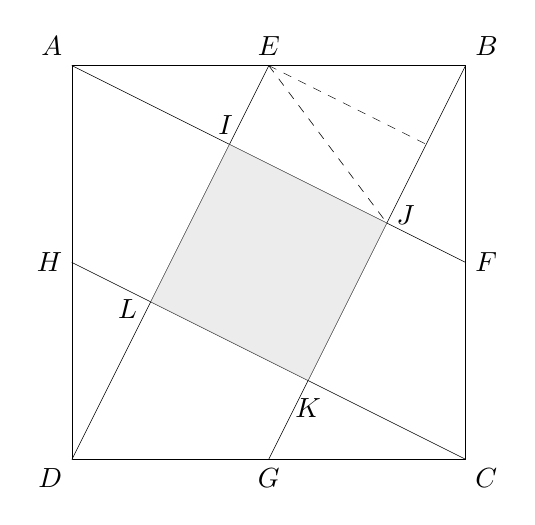
\begin{tikzpicture}[scale=1]
            \tkzDefPoint (0, 5){A}
            \tkzDefPoint (5, 5){B}
            \tkzDefPoint (5, 0){C}
            \tkzDefPoint (0, 0){D}
            \tkzDrawPolygon(A, B, C, D);

            \tkzLabelPoints[above left](A)
            \tkzLabelPoints[above right](B)
            \tkzLabelPoints[below right](C)
            \tkzLabelPoints[below left](D)

            \tkzDefMidPoint(A,B) \tkzGetPoint{E}
            \tkzDefMidPoint(B,C) \tkzGetPoint{F}
            \tkzDefMidPoint(C,D) \tkzGetPoint{G}
            \tkzDefMidPoint(D,A) \tkzGetPoint{H}
            \tkzLabelPoints[above](E)
            \tkzLabelPoints[right](F)
            \tkzLabelPoints[below](G)
            \tkzLabelPoints[left](H)

            \tkzDrawSegment(A, F)
            \tkzDrawSegment(H, C)
            \tkzDrawSegment(D, E)
            \tkzDrawSegment(G, B)

            \tkzInterLL(A,F)(E,D) \tkzGetPoint{I};
            \tkzInterLL(A,F)(G,B) \tkzGetPoint{J};
            \tkzInterLL(H,C)(G,B) \tkzGetPoint{K};
            \tkzInterLL(H,C)(E,D) \tkzGetPoint{L};
            \fill[opacity=0.5,color=gray!30] (I) -- (J) -- (K) -- (L) -- cycle;
            \tkzLabelPoints[above,xshift=-0.5mm](I)
            \tkzLabelPoints[right,yshift=1mm](J)
            \tkzLabelPoints[below,yshift=-1mm](K)
            \tkzLabelPoints[left,xshift=-0.5mm,yshift=-0.9mm](L);

            \tkzDrawSegment[dashed](E, J)

            \tkzDefLine[parallel=through E](I,J) \tkzGetPoint{X};
            \tkzInterLL(B,G)(E,X) \tkzGetPoint{X1};
            \tkzDrawSegment[dashed](E, X1)
        \end{tikzpicture}
        \end{center}
    \end{cbshadow}

    Draw a line parallel to AF through E and another line $\overline{EJ}$.
    It's easy to show that all 5 small triangles within $\triangle ABF$ are equal,
    because they all have same longest side and all angles are equal.
    Hence, the area of the small triangles is
    \begin{equation}
        {\mathlarger{\mathbb{A}}}_{AEI}
        = \frac{1}{5}{\mathlarger{\mathbb{A}}}_{ABF}
        = \frac{1}{5} \cdot \frac{1}{2} \cdot \frac{1}{2} \cdot 1
        = \frac{1}{20}\label{eq:smallarea}
    \end{equation}

    Then, the square area is
    \begin{equation}
        \begin{aligned}
            {\mathlarger{\mathbb{A}}}_{IJKL}
            &= {\mathlarger{\mathbb{A}}}_{EBDG} - 2 {\mathlarger{\mathbb{A}}}_{EBJI}\\
            &= {\mathlarger{\mathbb{A}}}_{EBDG} - 2 \cdot 3 \cdot {\mathlarger{\mathbb{A}}}_{AEI}\\
            &= {\mathlarger{\mathbb{A}}}_{EBDG} - 6 \cdot {\mathlarger{\mathbb{A}}}_{AEI}\\
            &= 1 \cdot \frac{1}{2} - 6 \cdot \frac{1}{20}\\
            &= \frac{1}{5}
        \end{aligned}\label{eq:square}
    \end{equation}
\end{document}
